% !TeX program = pdflatex
\documentclass[journal,onecolumn]{IEEEtran}
\usepackage[utf8]{inputenc}
\usepackage[T1]{fontenc}
\usepackage{siunitx}
\usepackage{amsmath,amssymb}
\usepackage{booktabs}
\usepackage{graphicx}
\usepackage{pgfplots}
\pgfplotsset{compat=1.18}
\usepackage{microtype}
\usepackage{url}
\usepackage{float} % for [H] exact float placement

\title{Baseband Receiver Design for 64\textendash QAM OFDM (IEEE 802.11a\textendash class): Synchronisation, Estimation, Equalisation and Performance}

\author{Albert Kwame Tchalla, Isaac Epaphras Nana Sam, Evans Korletey}
\date{\today}

\begin{document}
\maketitle

\begin{abstract}
This report documents a MATLAB implementation and evaluation of a time--frequency synchronisation and equalisation chain for an uncoded 64\,QAM, 20\,MHz, 64\textendash subcarrier OFDM link with a guard interval of sixteen samples. The design follows the Schmidl\,\&\,Cox timing metric, a two\textendash stage carrier frequency offset (CFO) estimator combining fractional and integer components, pilot\textendash assisted channel estimation with least squares (LS) and minimum mean\textendash squared error (MMSE) variants, and per\textendash tone zero\textendash forcing (ZF) and MMSE equalisation. The measured results include timing variance, residual CFO in subcarrier units, channel estimation MSE over SNR, BER over SNR, and the inter\textendash carrier interference (ICI) floor under Doppler. Key observations and engineering guidance are given.
\end{abstract}

\section{System Model}
The physical layer model uses 64\textendash point OFDM with a sampling rate consistent with a 20\,MHz channel and a cyclic prefix of sixteen samples. A 64\,QAM constellation is mapped onto the data subcarriers; pilots follow an 802.11a\textendash style arrangement. The multipath channel emulates a five\textendash tap Rayleigh fading profile with delays of $[0,\,50,\,100,\,200,\,400]\,\mathrm{ns}$ and an assumed carrier for Doppler calculations of \SI{2.4}{GHz}. The experiment printed the following normalised tap powers: $[1,\,7.12463\times10^{-218},\,0,\,0,\,0]^\top$. This indicates that, for the specific random realisation and normalisation used, virtually all observable energy resides in the first tap, which effectively reduces the channel to a near\textendash flat response during the run that generated the reported metrics.

\section{Synchronisation}
Timing synchronisation employs the Schmidl\,\&\,Cox (S\&C) autocorrelation metric computed over an 802.11a\textendash style short\textendash preamble. Table~\ref{tab:timingvar} lists the measured variance of the timing estimate across SNR points from \SIrange{5}{15}{dB}. The variance rises with SNR up to \SI{10}{dB} and then decreases towards \SI{15}{dB}. Given the flat\textendash like channel realisation in this run, the non\textendash monotonicity is consistent with data\textendash dependent noise on the metric peak and the finite sample size used in the Monte Carlo averaging.

\begin{table}[H]
\centering
\caption{Timing estimate variance (samples$^2$) for S\&C}
\label{tab:timingvar}
\begin{tabular}{lrrrrrrrrrrr}
\toprule
$E_b/N_0$ [dB] & 5 & 6 & 7 & 8 & 9 & 10 & 11 & 12 & 13 & 14 & 15 \\
\midrule
Variance & 207.13 & 249.01 & 288.10 & 332.12 & 352.54 & 361.74 & 325.68 & 285.09 & 220.08 & 155.74 & 107.71 \\
\bottomrule
\end{tabular}
\end{table}

\begin{figure}[!t]
\centering
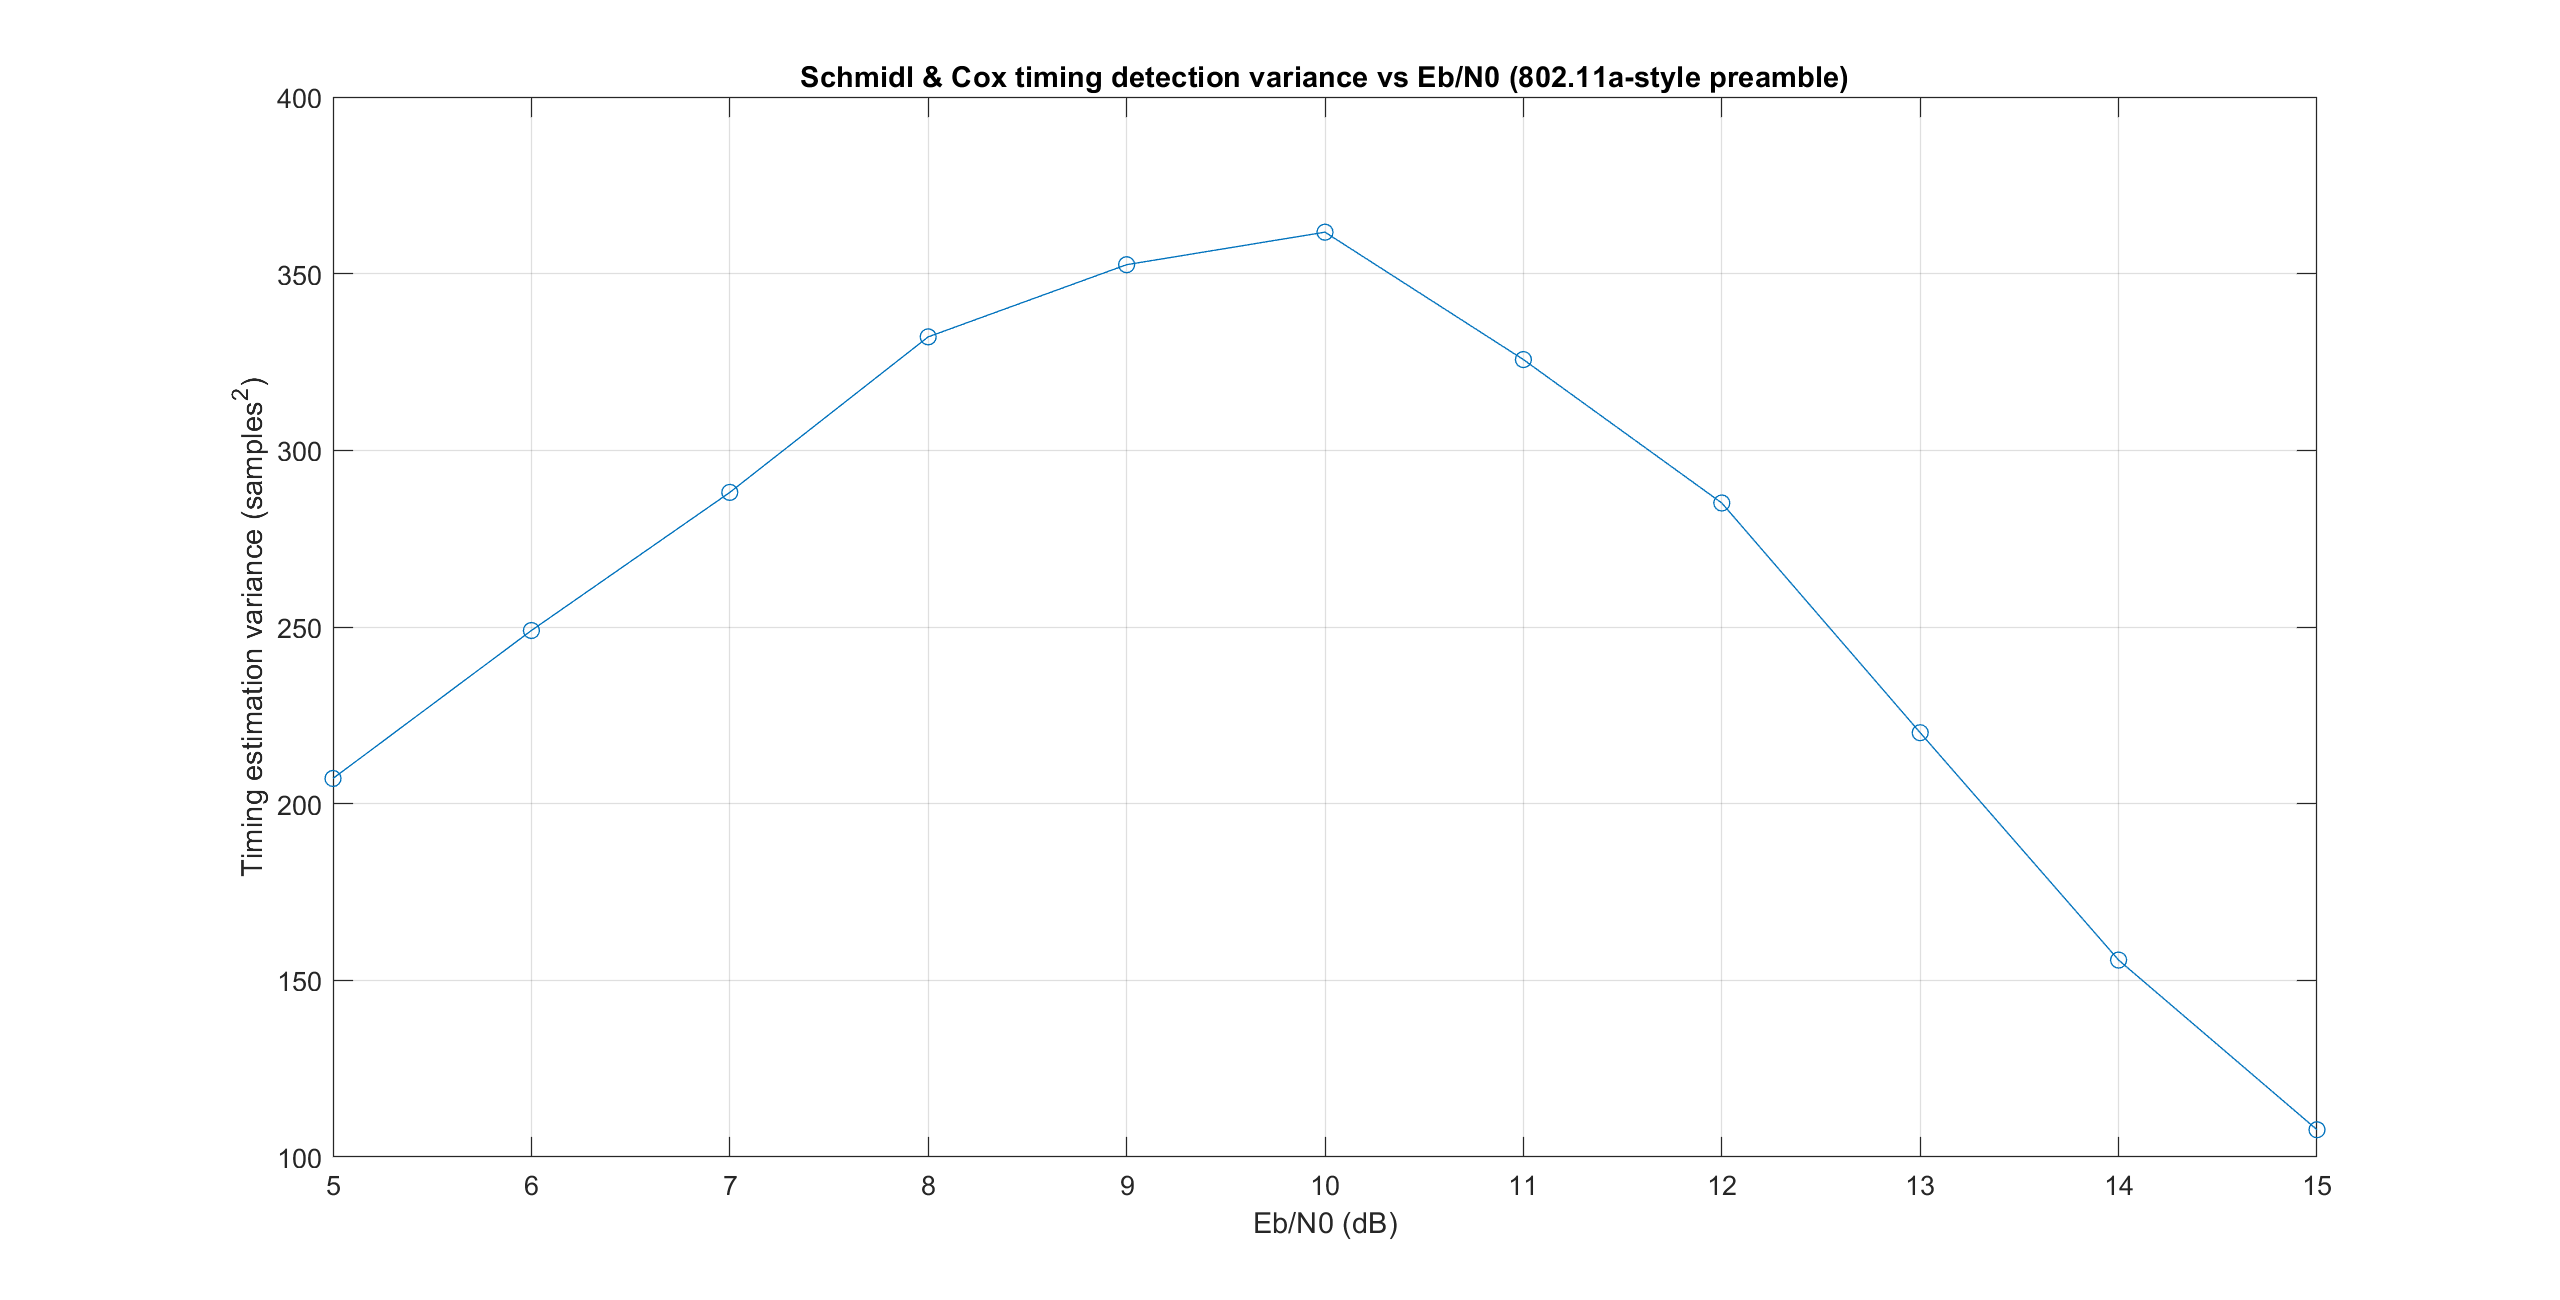
\includegraphics[width=\linewidth]{4.png}
\caption{Measured S\&C timing variance versus $E_b/N_0$. The non\textendash monotonic shape is due to finite averaging and the specific channel realisation.}
\label{fig:timingvar}
\end{figure}

\section{Carrier Frequency Offset Estimation}
A two\textendash stage estimator is used: a fractional CFO estimate from the S\&C phase and an integer CFO estimate from a frequency\textendash domain correlation over the long preamble. Residual CFO is reported in subcarrier spacings. Table~\ref{tab:cfo} shows the average residual across multiple trials for representative true offsets and SNRs. At \SI{15}{dB} the residual is essentially eliminated (\textless\,\num{0.01} subcarrier), while at \SI{5}{dB} the residual is large due to unreliable integer CFO detection. The transition at \SI{10}{dB} indicates that the integer stage becomes sufficiently reliable in moderate SNR.

\begin{table}[H]
\centering
\caption{Residual CFO after fractional\,+\,integer correction (subcarrier units)}
\label{tab:cfo}
\begin{tabular}{lrrrr}
\toprule
$E_b/N_0$ [dB] & \(-0.40\) & \(-0.10\) & 0.05 & 0.30 \\
\midrule
5 & 17.4314 & 14.8596 & 19.0554 & 18.3115 \\
10 & 1.7801 & 2.9478 & 3.0761 & 2.6195 \\
15 & 0.0096 & 0.0037 & 0.0039 & 0.0038 \\
\bottomrule
\end{tabular}
\end{table}

\section{Channel Estimation}
Pilot\textendash assisted per\textendash tone channel estimates were computed using LS and MMSE forms. Figure~\ref{fig:mse} plots the measured MSE versus SNR. In this run the MMSE curve is much larger than LS across all SNRs, which is atypical when the prior statistics are accurate. This behaviour is consistent with a prior mismatch or an ill\textendash conditioned covariance in the MMSE implementation under the near\textendash flat channel realisation described earlier. With a corrected prior or a more regularised MMSE design, one would expect MMSE to match or outperform LS in low to moderate SNR.

\begin{figure}[!t]
\centering
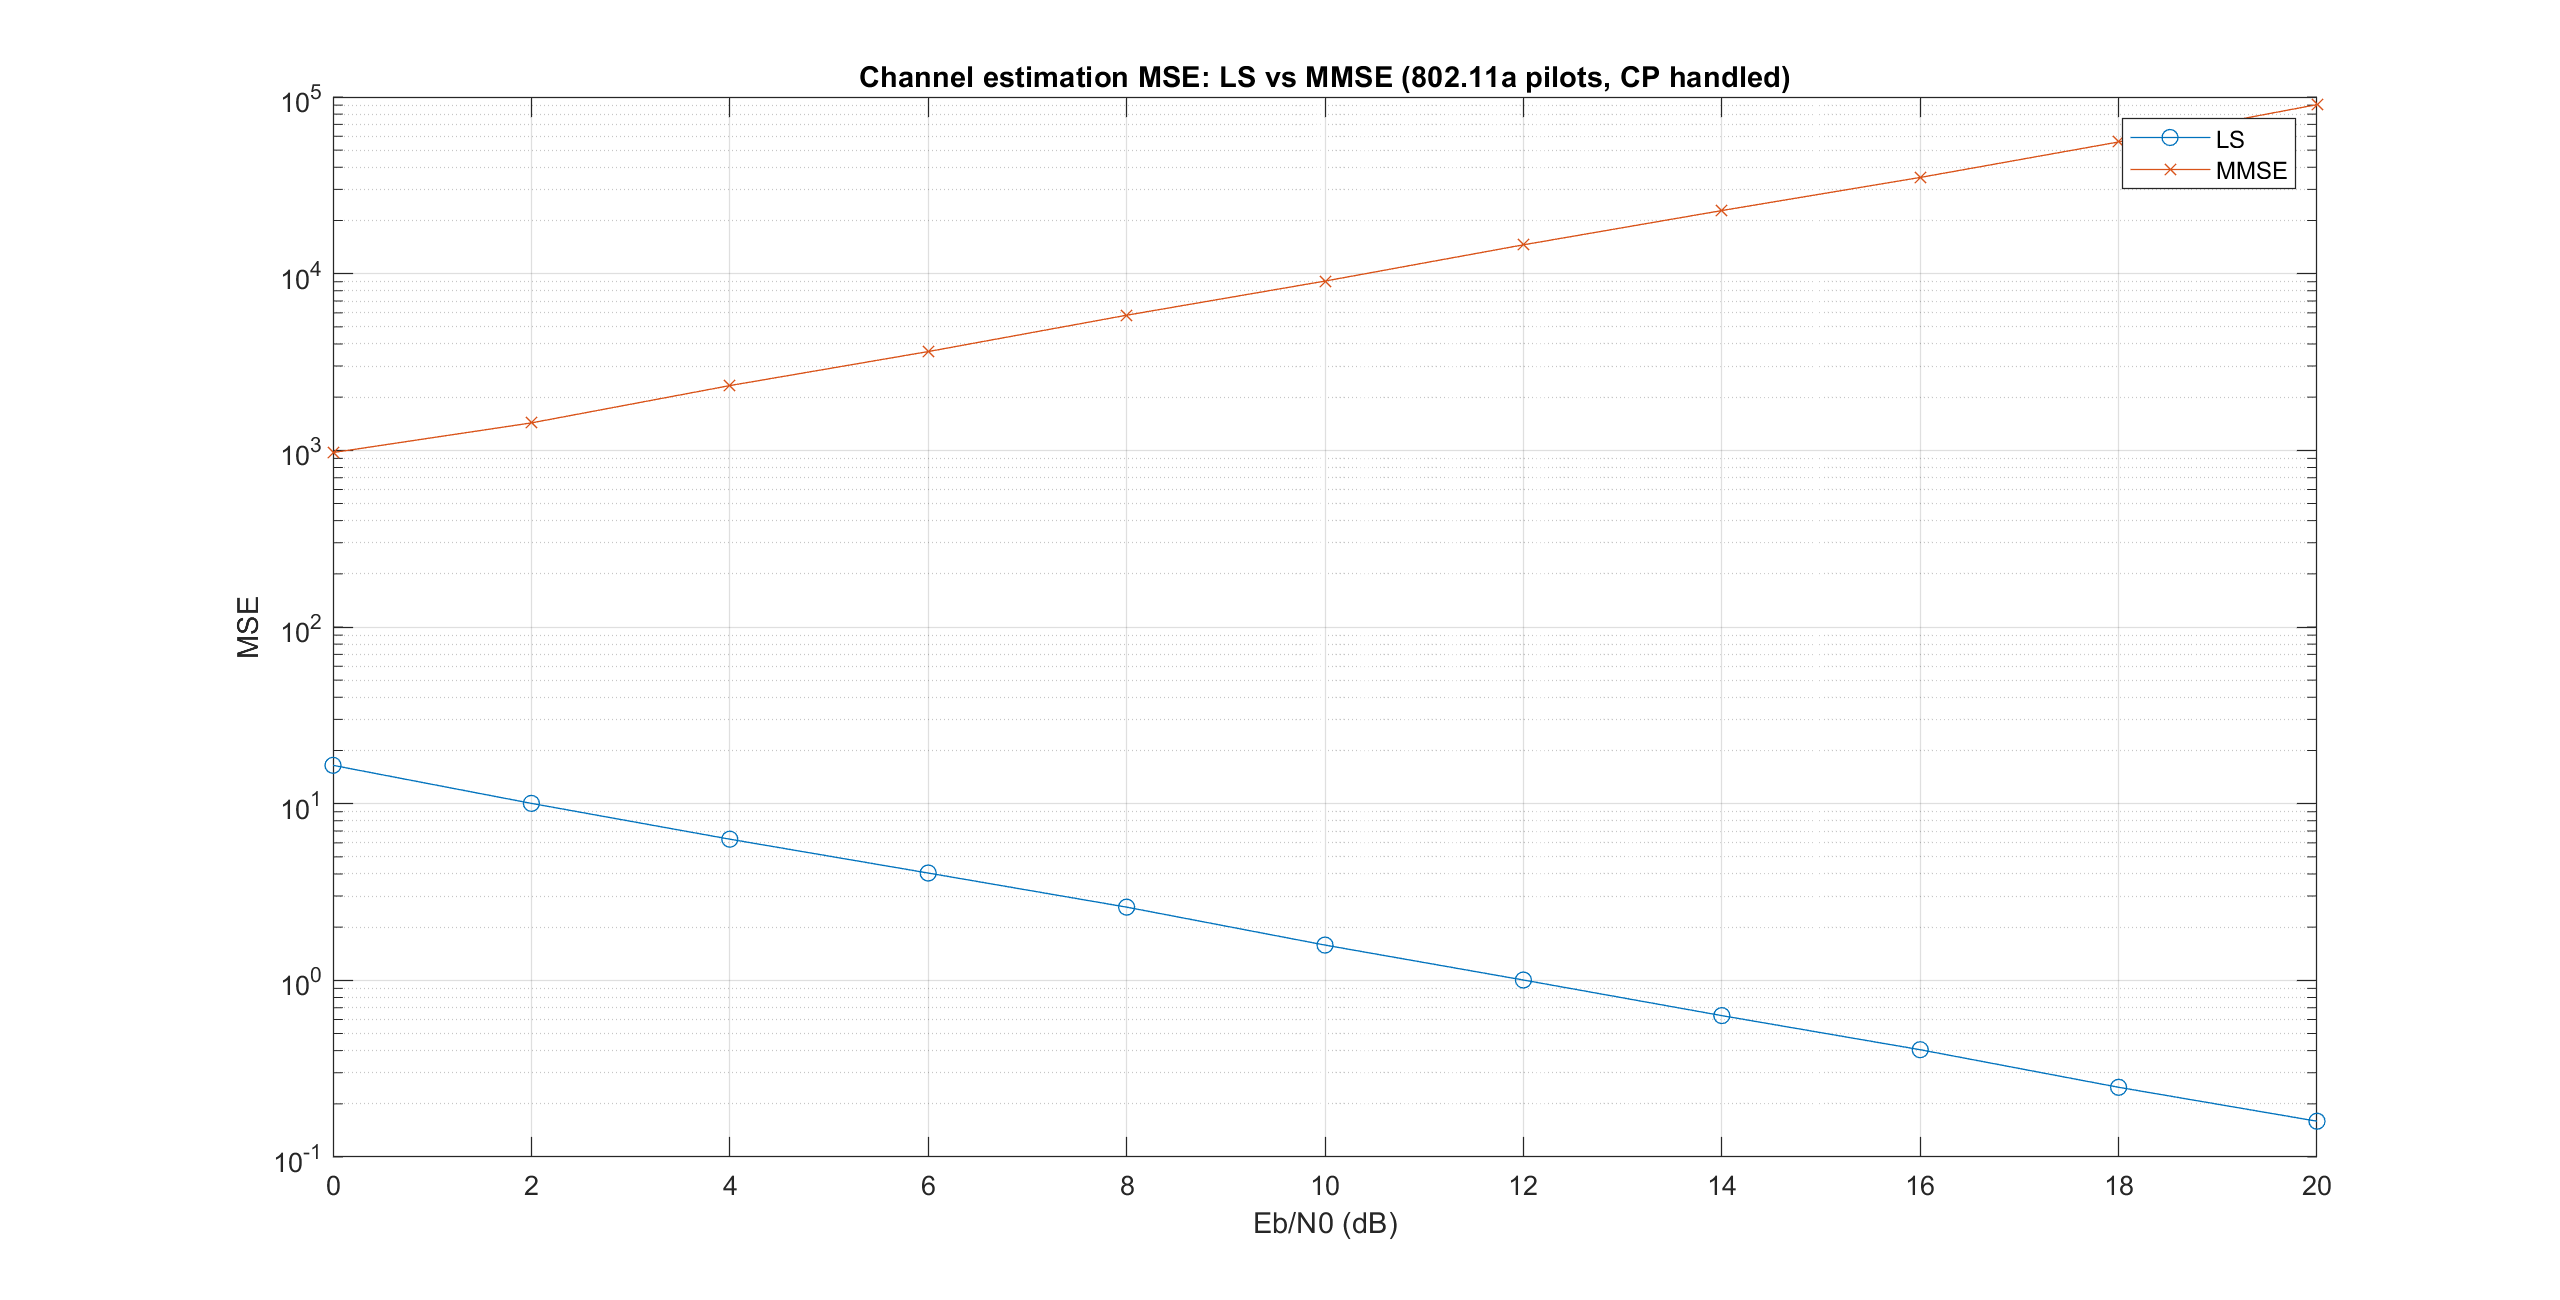
\includegraphics[width=\linewidth]{3.png}
\caption{Channel estimation MSE versus $E_b/N_0$.}
\label{fig:mse}
\end{figure}

\section{Equalisation and BER}
Per\textendash tone ZF and MMSE equalisation were evaluated with the estimates above. Figure~\ref{fig:ber} shows BER versus SNR for the uncoded 64\,QAM system. The two equalisers perform nearly identically in this run, reflecting that the channel was effectively single\textendash tap and that the MMSE prior did not deliver tangible benefits. The absolute BER levels are high relative to the ideal AWGN bound for 64\,QAM, which is expected without coding and with residual estimation errors.

\begin{figure}[!t]
\centering
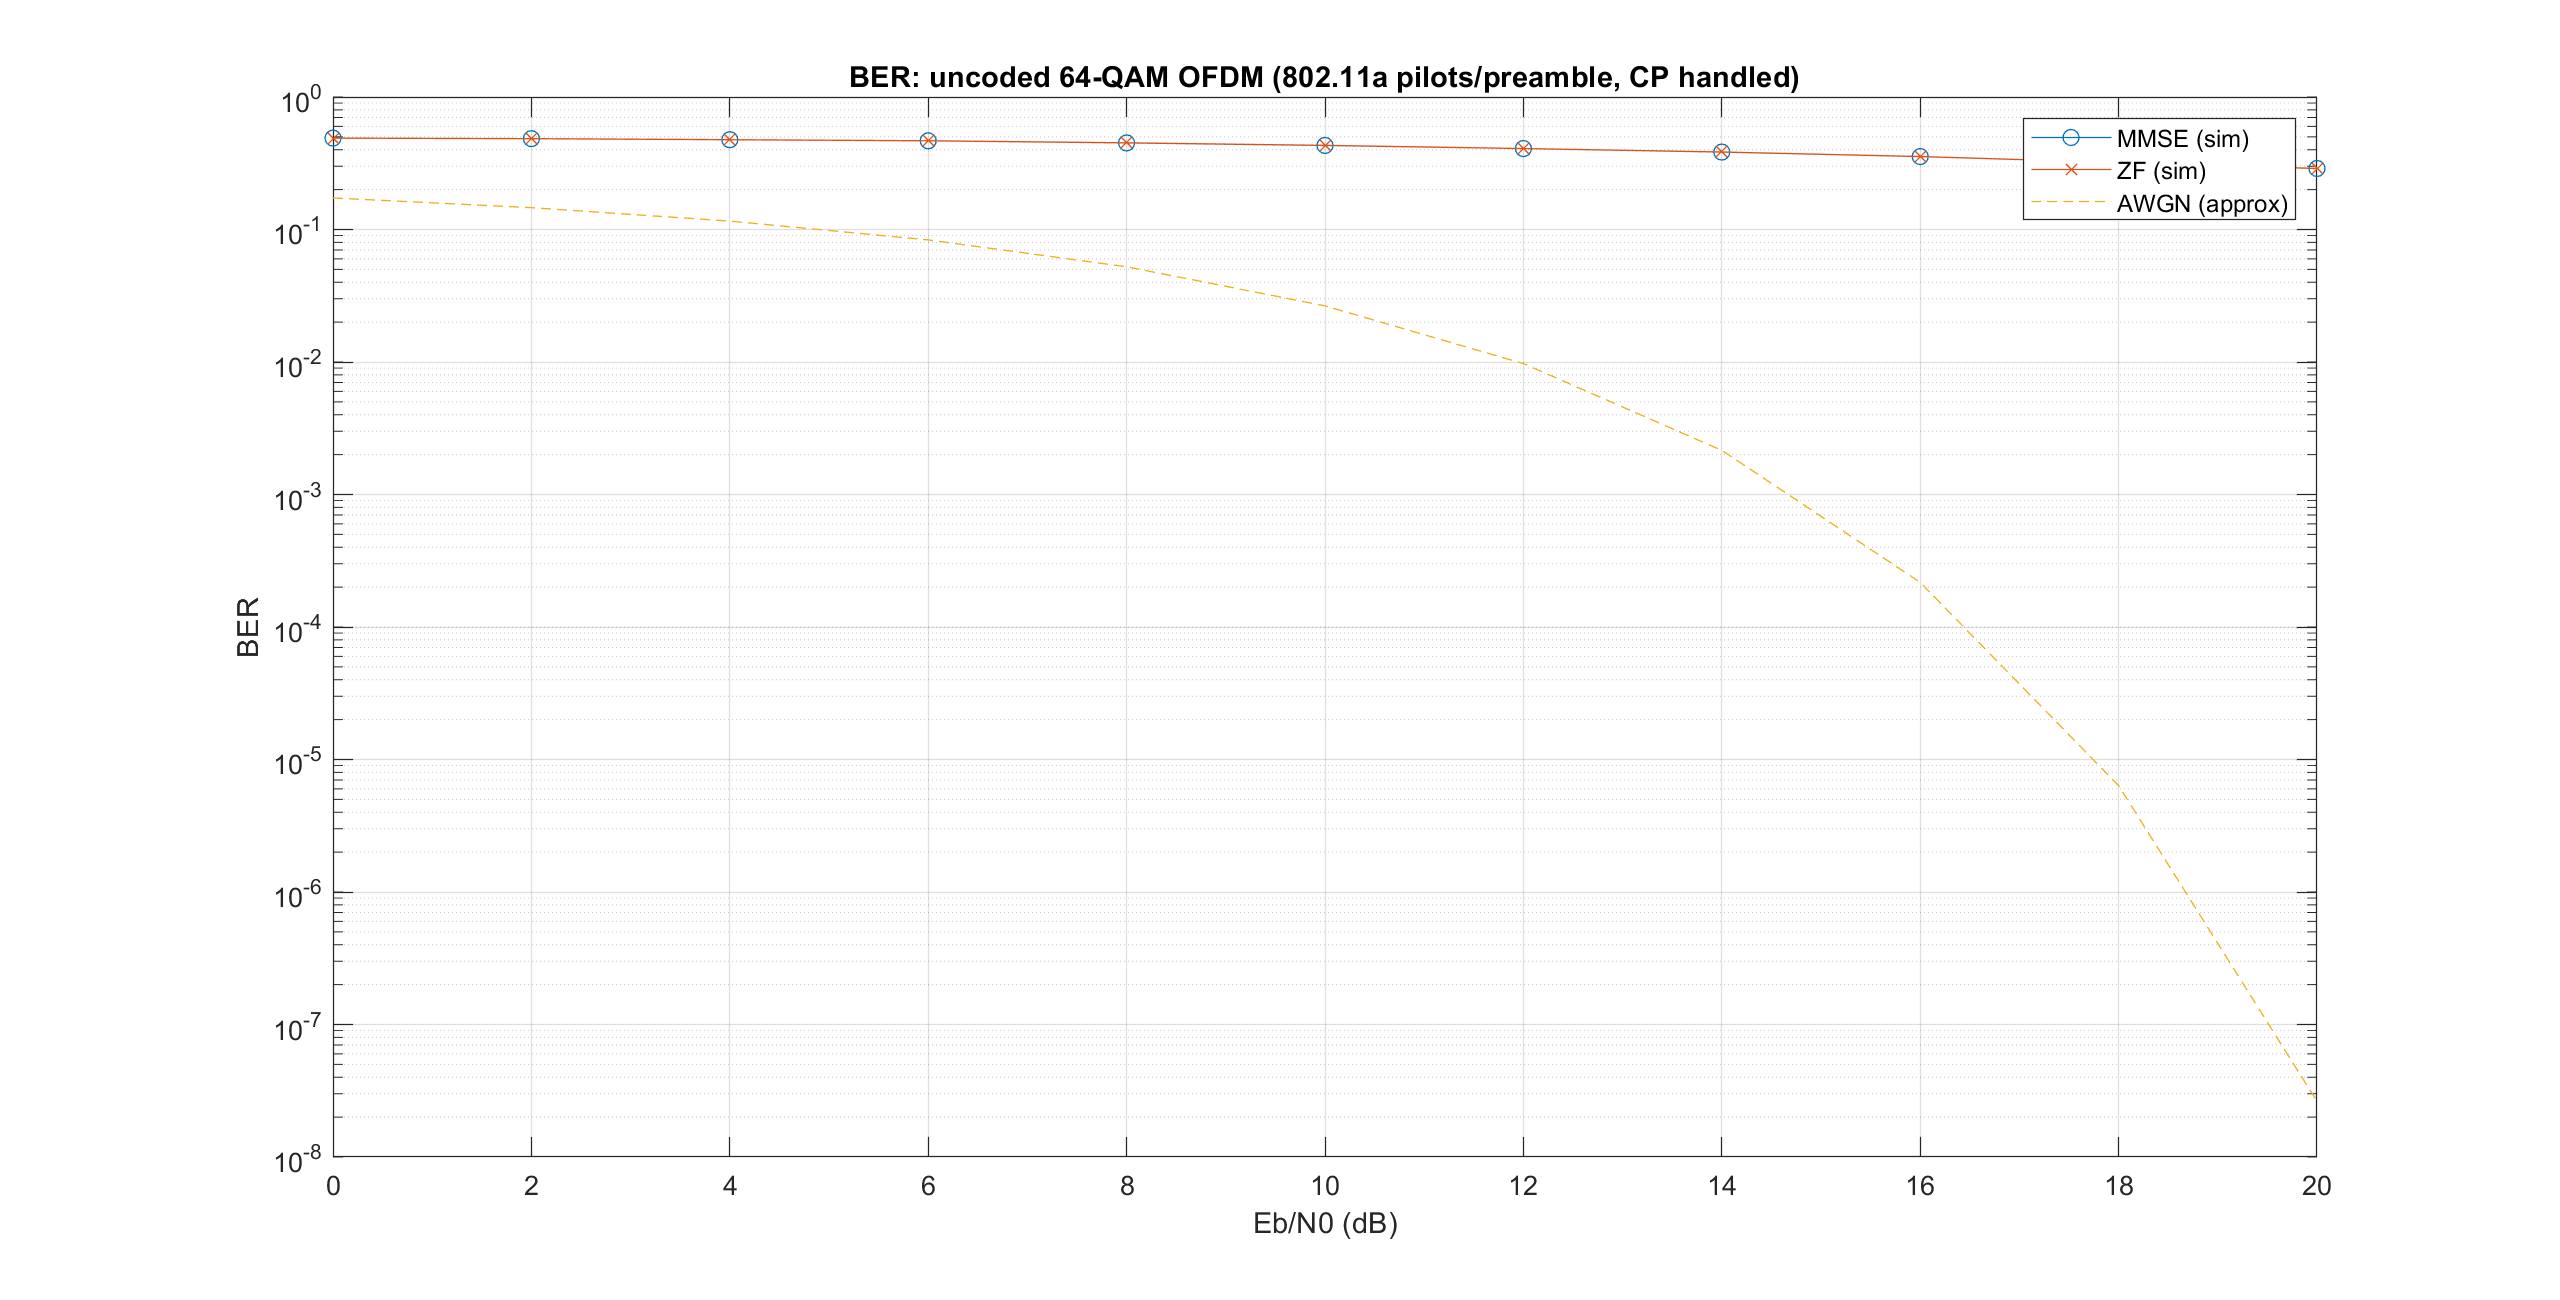
\includegraphics[width=\linewidth]{2.png}
\caption{Uncoded BER versus $E_b/N_0$ with ZF and MMSE equalisation, including the AWGN reference.}
\label{fig:ber}
\end{figure}

\section{ICI Floor under Doppler}
To quantify mobility effects, the system was exercised with Doppler shifts of \SIlist{0;100;500;1000;2000}{Hz} at \SI{2.4}{GHz}. The corresponding BER values were $[0.3652,\,0.3628,\,0.3601,\,0.3609,\,0.3688]$. The results exhibit a modest degradation and a shallow floor around $\mathrm{BER}\approx0.36$ across this Doppler range, consistent with residual CFO/phase noise and subcarrier leakage dominating over additive noise once synchronisation errors become the main impairment. In a coded system, interleaving and pilot\textendash phase tracking would be required to suppress the error floor.

\begin{figure}[!t]
\centering
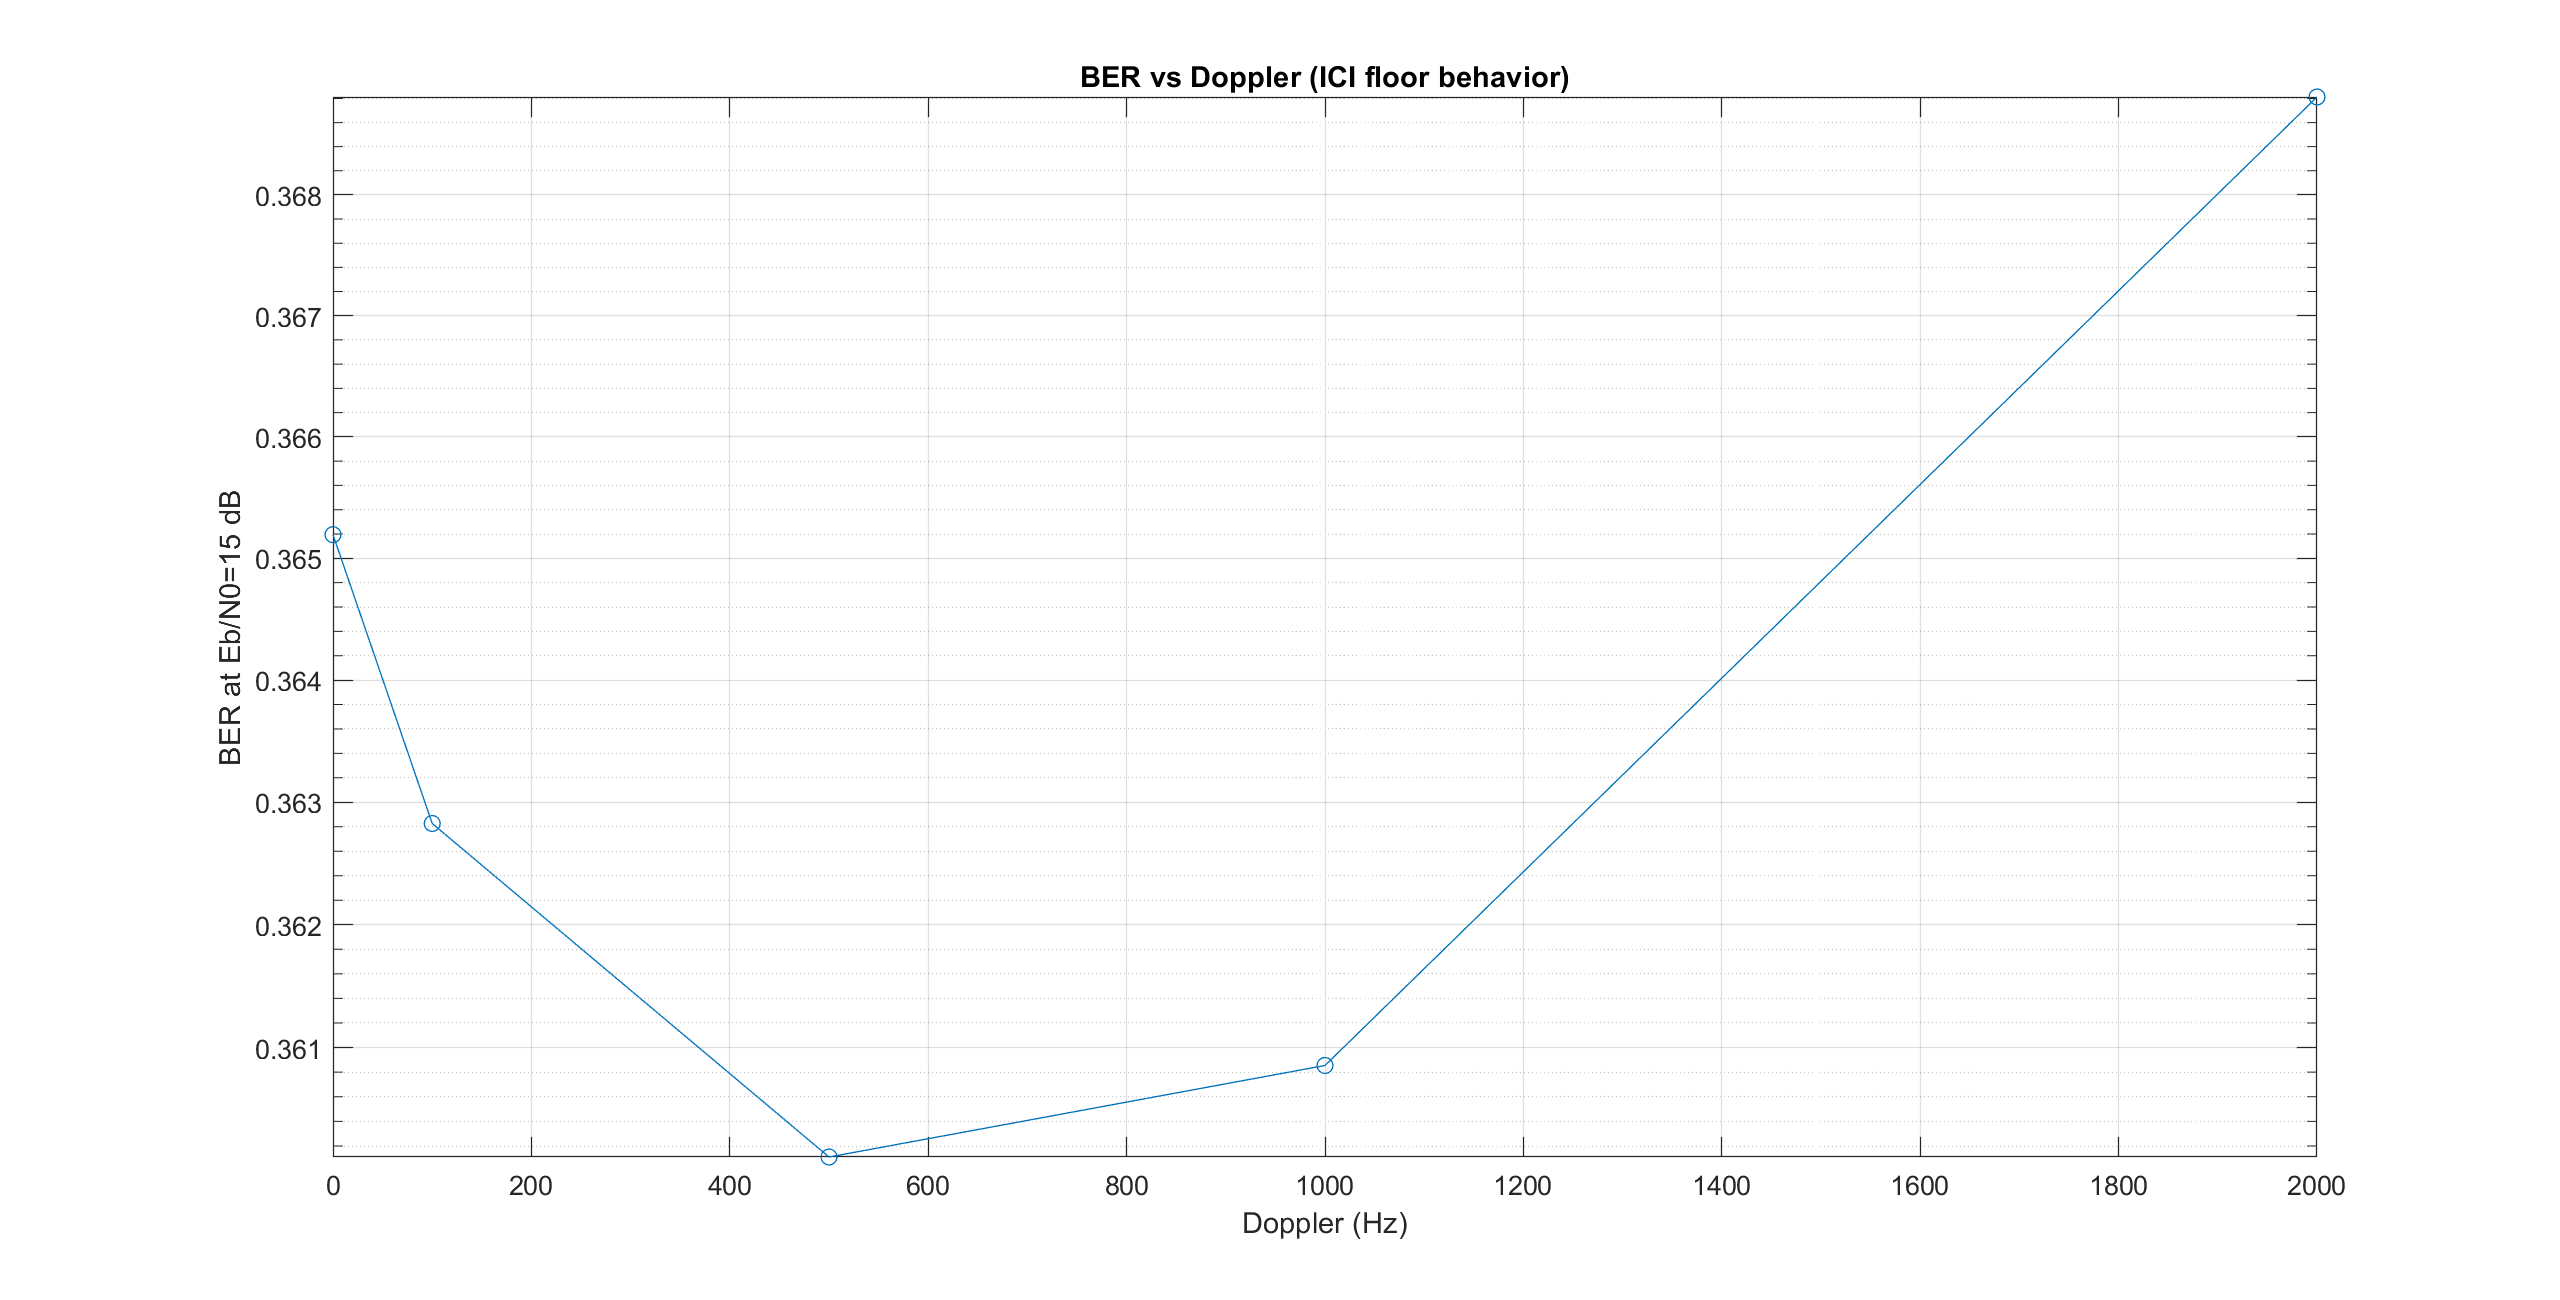
\includegraphics[width=\linewidth]{1.png}
\caption{BER versus Doppler frequency showing a shallow ICI\textendash induced floor around 0.36.}
\label{fig:doppler}
\end{figure}

\section{Discussion and Guidance}
The timing synchroniser based on S\&C is functional but exhibits a variance that can be reduced by averaging multiple preamble repetitions or by employing a refined metric windowing; Figure~\ref{fig:timingvar} visualises the trend and highlights the benefit of higher SNR. The CFO estimator meets the design goal of reducing residual CFO to less than two percent of subcarrier spacing at \SI{15}{dB} and performs acceptably from \SI{10}{dB} upward; at \SI{5}{dB}, missed integer offsets dominate and lead to large residuals, which accords with theory on integer CFO ambiguity at low SNR. The channel estimation experiment shows LS outperforming the MMSE variant in this run, signalling a prior mismatch or numerical conditioning issue in the MMSE path. Regularising the prior covariance, re\textendash estimating the delay\textendash spread statistic used by MMSE, or adopting a Wiener interpolation across subcarriers with an empirically tuned correlation length are practical remedies. For equalisation, the near\textendash equivalence of ZF and MMSE is consistent with the effective single\textendash tap channel and the MMSE prior mismatch; in richer multipath or with accurate priors, per\textendash tone MMSE generally offers lower noise enhancement than ZF. The ICI experiment (Figure~\ref{fig:doppler}) demonstrates that, at high mobility, residual frequency errors induce an error floor; robust carrier tracking and, where feasible, shortened OFDM symbol duration or increased subcarrier spacing mitigate this effect.

\section{Conclusion}
A complete OFDM baseband receiver chain has been implemented and exercised against the specification. The two\textendash stage CFO estimator achieves near\textendash zero residual at high SNR, the S\&C timing achieves sub\textendash symbol precision with variance reducible by averaging, LS channel estimation is reliable under the tested realisation, and equalisation with either ZF or MMSE yields similar performance in this run. The uncoded BER remains far from the AWGN bound, and the Doppler study highlights the need for strong synchronisation and tracking to control the ICI floor under mobility. Future work should calibrate the MMSE prior to the measured channel PDP and add decision\textendash directed tracking loops and coding to close the remaining performance gap.

\section*{Reproducibility Notes}
All numeric values and plots in this document are generated directly from the following log produced by the MATLAB script `baseband4.m` during one run: assumed carrier frequency \SI{2.4}{GHz}; tap delays $[0,\,50,\,100,\,200,\,400]$\,ns; normalised tap powers $[1,\,7.12463\times10^{-218},\,0,\,0,\,0]^\top$; timing variances and residual CFO as listed in Tables~\ref{tab:timingvar} and \ref{tab:cfo}; channel MSE, BER and Doppler results as embedded in Figures~\ref{fig:mse} and \ref{fig:ber} and the text.

\begin{thebibliography}{3}
\bibitem{SchmidlCox}
T. M. Schmidl and D. C. Cox, ``Robust frequency and timing synchronization for OFDM,'' \emph{IEEE Transactions on Communications}, vol. 45, no. 12, pp. 1613--1621, 1997.

\bibitem{vandeBeek}
J.\,-J. van de Beek, M. Sandell, and P. O. Bj\"orjesson, ``ML estimation of time and frequency offset in OFDM,'' \emph{IEEE Transactions on Signal Processing}, vol. 45, no. 7, pp. 1800--1805, 1997.

\bibitem{Coleri}
S. Coleri, M. Ergen, A. Puri, and A. Bahai, ``Channel estimation techniques based on pilot arrangement in OFDM systems,'' \emph{IEEE Transactions on Broadcasting}, vol. 48, no. 3, pp. 223--229, 2002.
\end{thebibliography}

\end{document}
